\documentclass[12pt,a4paper]{article}
\usepackage{ucs}
\usepackage[utf8x]{inputenc}
\usepackage{amsmath}
\usepackage{graphicx}
\usepackage{wrapfig}
\usepackage{trfsigns}

\title{Osnove Mehatronike 4. lab}
\newcommand{\brvjezbe}{3}
\newcommand{\ime}{Niko Višnjić}
\newcommand{\jmbag}{0036449299}
\newcommand{\grupa}{unknown}
\newcommand{\predmet}{Osnove mehatronike} 
\newcommand{\fakultet}{Fakultet elektrotehnike i računarstva Zagreb} 
\newcommand{\zavod}{Zavod za elektrostrojarstvo i automatizaciju } 
\newcommand{\imevjezbe}{Vježba 4: Regulacija pozicije rotacijskog elektromehaničkog sustava SRV02 
\newline-sinteza regulatora-}
\usepackage[hmargin={3.5cm,2.5cm},height=25.5cm]{geometry}
\input{"zaglavlje.tex"}
\setcounter{secnumdepth}{4}

\DeclareMathSizes{12}{12}{10}{12}

\begin{document}
\section{Uvod}
U okviru ove vježbe obavljamo sintezu regulatora pozicije rotacijskog elektromehaničkog sustava SRV02 i njegovu simulaciju na par specifičnih primjera.
\newline

Vježba se sastoji od dva pokusa.


U sklopu prvog pokusa obavljamo sintezu regulatora pozicije osovine rotacijskog elektromehaničkog sustava SRV02 korištenjem Matlab funkcija.

Postupak sinteze uključuje:

\begin{itemize}
  \item Određivanje matematičkog modela rotacijskog elektromehaničkog sustava SRV02 iz zadanih zahtjeva
  \item Simulaciju matematičkog modela rotacijskog elektromehaničkog sustava SRV02 unutar Simulink programskog okruženja 
  \item projektiranje PV regulatora pozicije osovine prema zadanim regulacijskim
zahtjevima iznosa i vremena prvog nadvišenja 
\end{itemize}

U sklopu drugog pokusa obavljamo simulaciju kruga regulacije pozicije u Simulinku u svrhu provjere ispravnosti parametara regulatora dobivenih sintezom
\newline 

U nastavku dokumentiramo i opisujemo pokuse te bilježimo dobivene rezultate i naša zapažanja iz dobivenih mjerenja.

\newpage

\section{Pokusi}
\subsection{Pokus 1: Određivanje parametara PV regulatora pozicije rotacijskog elektromehaničkog sustava SRV02}

Zadatak je projektirati regulator pozicije rotacijskog elektromehaničkog sustava  SRV02, koji će zadovoljiti zadane regulacijske zahtjeve, poglavlje ~\ref{sec:zahtjevi}. 

Krećemo od matematičkog modela rotacijskog modula kojeg smo izveli u sklopu 2. laboratorijske vježbe.

\subsubsection{Matematički model rotacijskog elektromehaničkog sustava SRV02}
Uzevši u obzir zakone kinematike te korištenjem Kirchhoffovih zakona za električki model motora prikazan na slici 2.1, i primjenom određenih zanemarenja, dobivamo sljedeći sustav jednadžbi.

\begin{figure}[h]
	\begin{center}
	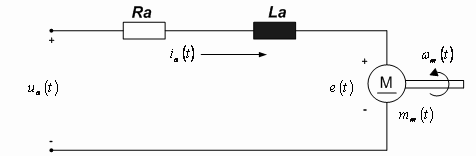
\includegraphics[width=0.8\textwidth] {ele_motor.png}
    \caption{Nadomjesna shema naponom upravljanog istosmjernog motora}
    \end{center}
\end{figure}

\begin{equation}
 i_a=\frac{u_a-k_e\omega_m}{R_a}
\end{equation}

\begin{equation}
 J_m\frac{\mathrm{d}\omega_m}{\mathrm{d}t}=m_m - \frac{m_t}{\eta_gK_g}
\end{equation}

\begin{equation}
J_t\frac{\mathrm{d}\omega_t}{\mathrm{d}t}=m_t - B_{eq}\omega_t
\end{equation}

Iz sustava jednadžbi slijedi prijenosna funkcija prvog reda koja opisuje rotacijski elektromehanički sustav:

\begin{equation}
G(s)=\frac{\omega_t(s)}{u_a(s)}=\frac{\eta_g\eta_mk_mK_g}{J_{eq}R_as + B_{eq}R_a+\eta_g\eta_mk_ek_mK_g^2}
\end{equation}

gdje \begin{equation}J_{eq}=J_t+\eta_gJ_mK_g^2\end{equation}
Izraz (2-5) opisuje ukupni (ekvivalentni) moment inercije reduciran na stranu tereta.
\newline

Kako vrijedi da je ovisnost pozicije i brzine okreta:

\begin{equation}
\frac{\mathrm{d}^2\varepsilon_t}{\mathrm{d}t^2} = \omega_m
\end{equation}
\newpage


Tražena prijenosna funkcija koja opisuje ovisnost pozicije, odnosno kuta zakreta osovine oko rotacijske osi, s obzirom na napon armature je kako slijedi:

\begin{equation}
G_m(s)=\frac{\varepsilon_t(s)}{u_a(s)}=\frac{\eta_g\eta_mk_mK_g}{J_{eq}R_as^2 + (B_{eq}R_a+\eta_g\eta_mk_ek_mK_g^2)s}
\end{equation}

Matematički model elektromehaničkog sustava SRV02 koji smo dobili proračunom prikazujemo unutar Simulink okruženja pomoću odgovarajuće nadomjesne sheme. Nadomjesnu shemu možemo vidjeti na slici 2.2.

\begin{figure}[h]
	\begin{center}
	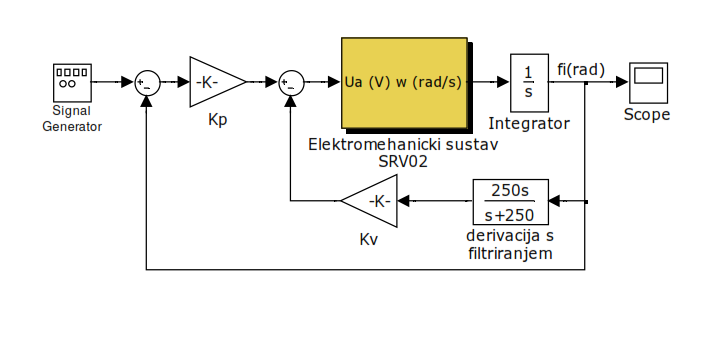
\includegraphics[width=0.8\textwidth] {nadomjesni_model.png}
    \caption{Simulink model elektromehaničkog rotacijskog sustava SRV02}
    \end{center}
\end{figure}

\subsubsection{Regulacijski zahtjevi}
\label{sec:zahtjevi}
Zadatak je projektirati sustav regulacije pozicije pomoću PV regulatora s ciljem upravljanja rotacijskim elektromehaničkim sustavom SVR02 sa sljedećim zahtjevima:

\begin{itemize}
  \item Sustav treba imati nadvišenje manje od 5\% ($\sigma_m = 0.05$)
  \item Vrijeme prvog maksimuma mora biti 100 ms ($t_p = 0.100$)
  
\end{itemize}


\subsubsection{Projektiranje PV regulatora pozicije}

Cilj ove vježbe je projektiranje regulatora pozicije rotacijskog elektromehaničkog modula SRV02. Za razliku od modela iz vježbe 2., nije potrebno integralno pojačanje regulatora, jer je isto sadržano u funkciji zatvorenog kruga, u što se možemo uvjeriti pogledom na jednadžbu (2-7). Uzimajući to u obzir, te s namjerom da pojednostavimo sintezu, koristit ćemo regulator stanja (engl. state feedback controller), tj. regulator koji koristi jedinstveni regulator (pozicije i brzine) s dostupnim (mjerljivim ili estimiranim) varijablama stanja sustava. Za ovaj slučaj to su pozicije brzine (engl. \textbf{P}osition and \textbf{V}elocity), pa se ovakav regulator stanja zove i \textbf{PV} regulator . Upravljački algoritam PV regulatora ima sljedeći oblik:

\begin{equation}
u_a = - K_p(\varepsilon_t - \varepsilon_d) - K_v\frac{\mathrm{d}\varepsilon_t}{\mathrm{d}t}
\end{equation}

\newpage


Sustav kojeg smo matematički modelirali povezujemo s PV regulatorom nadomjesnom shemom u Simulink okruženju kao što je prikazano na slici 2.3.

\begin{figure}[h]
	\begin{center}
	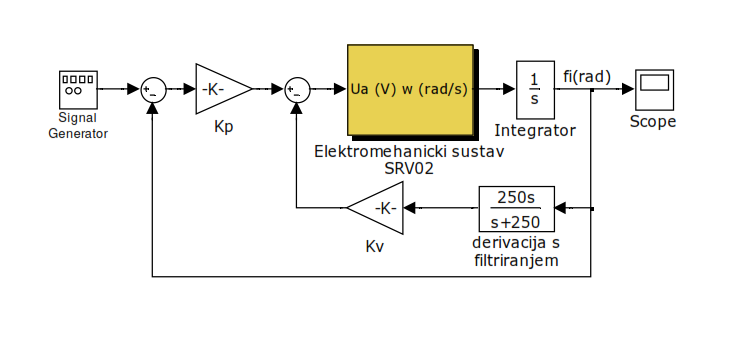
\includegraphics[width=0.8\textwidth] {PV_model.png}
    \caption{Nadomjesni model elektromehaničkog sustava SRV02 s PV regulatorom}
    \end{center}
\end{figure}

Na osnovu trenutnih saznanja možemo pristupiti sintezi PV regulatora koristeći prijenosnu funkciju drugog reda, čiji opći oblik glasi

\begin{equation}
G(s) = \frac{\omega_n^2}{s^2+2\zeta\omega_ns+\omega_n^2}
\end{equation}

s karakterističnom jednadžbom:

\begin{equation}
s^2+2\zeta\omega_ns+\omega_n^2 = 0
\end{equation}

  

Prijenosnu funkciju zatvorenog kruga regulacije dobivamo iz relacija (2-7) i (2-8), te ona glasi:

\begin{equation}
G(S) = \frac{\varepsilon_t(s)}{\varepsilon_d(s)}
\end{equation}

Na osnovi karakteristične jednadžbe te zadanih kriterija potrebno je odrediti parametre PV regulatora ($K_p$ i $K_v$).Da bi mogli odrediti parametre regulatora, moramo najprije izračunati vrijednosti prirodne frekvencije $\omega_n$ te prigušenja $\zeta$, koji se određuju prema kriterijima zadanim u poglavlju ~\ref{sec:zahtjevi}.

Prigušenje $\zeta$, računamo iz sljedećeg izraza, gdje nadvišenje znamo prema kriterijima regulatora da iznosi $\omega_n = 0.05$:


\begin{equation}
\sigma_m = e^{\frac{-\zeta\pi}{\sqrt{1-\zeta^2}}} \Rightarrow \zeta = \sqrt{\frac{ln^2\sigma_m}{\pi^2 + ln^2\sigma_m}} = 0.6901 
\end{equation}

Korištenjem upravo izračunatog iznosa prigušenja $\zeta$ te poznatog nam kriterija za vrijeme prvog maksimuma koje iznosi $t_p = 0.100$, računamo prirodnu frekvenciju $\omega_n$ iz sljdećih jednadžbi:

\begin{equation}
t_p = \frac{\pi}{\omega_n\sqrt{1-\zeta^2}} \Rightarrow \omega_n = \frac{\pi}{t_p\sqrt{1-\zeta^2}} = 43.4098 \mathrm{rad\\s}
\end{equation}

\newpage

Svodimo prijenosnu funkciju zatvorenog kruga regulacije pozicije G(s) na oblik prikazan jednadžbom (2-9). Krećemo od izraza (2-8)

\begin{equation}
u_a = - K_p(\varepsilon_t - \varepsilon_d) - K_v\frac{\mathrm{d}\varepsilon_t}{\mathrm{d}t} \quad  \laplace \quad U_a(s) = -K_p(\varepsilon_t(s) - \varepsilon_d(s)) - K_v \cdot s \cdot \varepsilon_t(s)
\end{equation}

Slijedi


\begin{equation}
\frac{U_a(s)}{\varepsilon_t(s)} + (K_p - K_v \cdot s) = K_p \frac{\varepsilon_d(s)}{\varepsilon_t(s)} 
\end{equation}

Kako znamo da vrijedi

\begin{equation}
G(S) = \frac{\varepsilon_t(s)}{\varepsilon_d(s)}
\end{equation}

te mozemo zapisati $G_m(s)$ na sljedeci način

\begin{equation}
G_m(s)=\frac{\varepsilon_t(s)}{u_a(s)}=\frac{\eta_g\eta_mk_mK_g}{J_{eq}R_as^2 + (B_{eq}R_a+\eta_g\eta_mk_ek_mK_g^2)s} = \frac{K}{Ts^2+s}
\end{equation}

Sređivanjem i korištenjem izraza (2-18) i (2-19) u (2-17) dobivamo traženu prijenosnu funkciju svedenu na oblik prikazan jednadžbom (2-9). Prijenosna funkcija je data sljedećim izrazom:

\begin{equation}
G(s) = \frac{K_p}{G_m(s)^{-1} + K_vs + K_p} = \frac{K\cdot K_p}{Ts^2 + (K\cdot K_v + 1)s + K\cdot K_p}
\end{equation}

Usporedimo li tu jednadžbu s jednadžbom (2-9)

\begin{equation}
G(s) = \frac{\omega_n^2}{s^2+2\zeta\omega_ns+\omega_n^2}
\end{equation}

odnosno s karakterističnom jednadžbom:

\begin{equation}
s^2+2\zeta\omega_ns+\omega_n^2 = 0
\end{equation}


Možemo očitati sljedeće relacije:

\begin{subequations}
\begin{align}
	K_p &= \frac{T\omega_n^2}{K} \\
	K_v &= \frac{2\zeta\omega_nT -1}{K}
\end{align}
\end{subequations}

Vrijednosti T i K lako izračunamo, te dobivamo sljedeće vrijednosti za date parametre regulacije:


\begin{subequations}
\begin{align}
	K &= \frac{\eta_g\eta_mk_mK_g}{B_{eq}R_a+\eta_g\eta_mk_ek_mK_g^2} = 1.7588\\
	T &= \frac{J_{eq}R_a}{B_{eq}R_a+\eta_g\eta_mk_ek_mK_g^2} = 0.0274
\end{align}
\end{subequations}

\newpage

Te naposljetku uvrštavanjem dobivamo tražene parametre PV regulatora.

\begin{subequations}
\begin{align}
	K_p &= \frac{T\omega_n^2}{K} = 29.3399\\
	K_v &= \frac{2\zeta\omega_nT -1}{K} = 0.3643
\end{align}
\end{subequations}

Time je sinteza regulatora završena te isti treba testirati simulacijom u MATLAB/Simulink okruženju.


\subsection{Pokus 2: Simulacija kruga regulacije pozicije rotacijskog elektromehaničkog sustava SRV02}

Nakon određivanja parametara regulatora potrebno je simulirati krug regulacije pozicije osovine rotacijskog elektromehaničkog modula SRV02, kako bi se potvrdilo da taj krug ispunjava postavljene kriterije u poglavlju ~\ref{sec:zahtjevi}. 


\subsubsection{Simulacijski model}
U Simulink okruženju konstruiramo odgovarajući simulacijski model sustava regulacije pozicije rotacijskog elektromehaničkog modula SRV02, kojeg možemo vidjeti na slici 2.4.

\begin{figure}[h]
	\begin{center}
	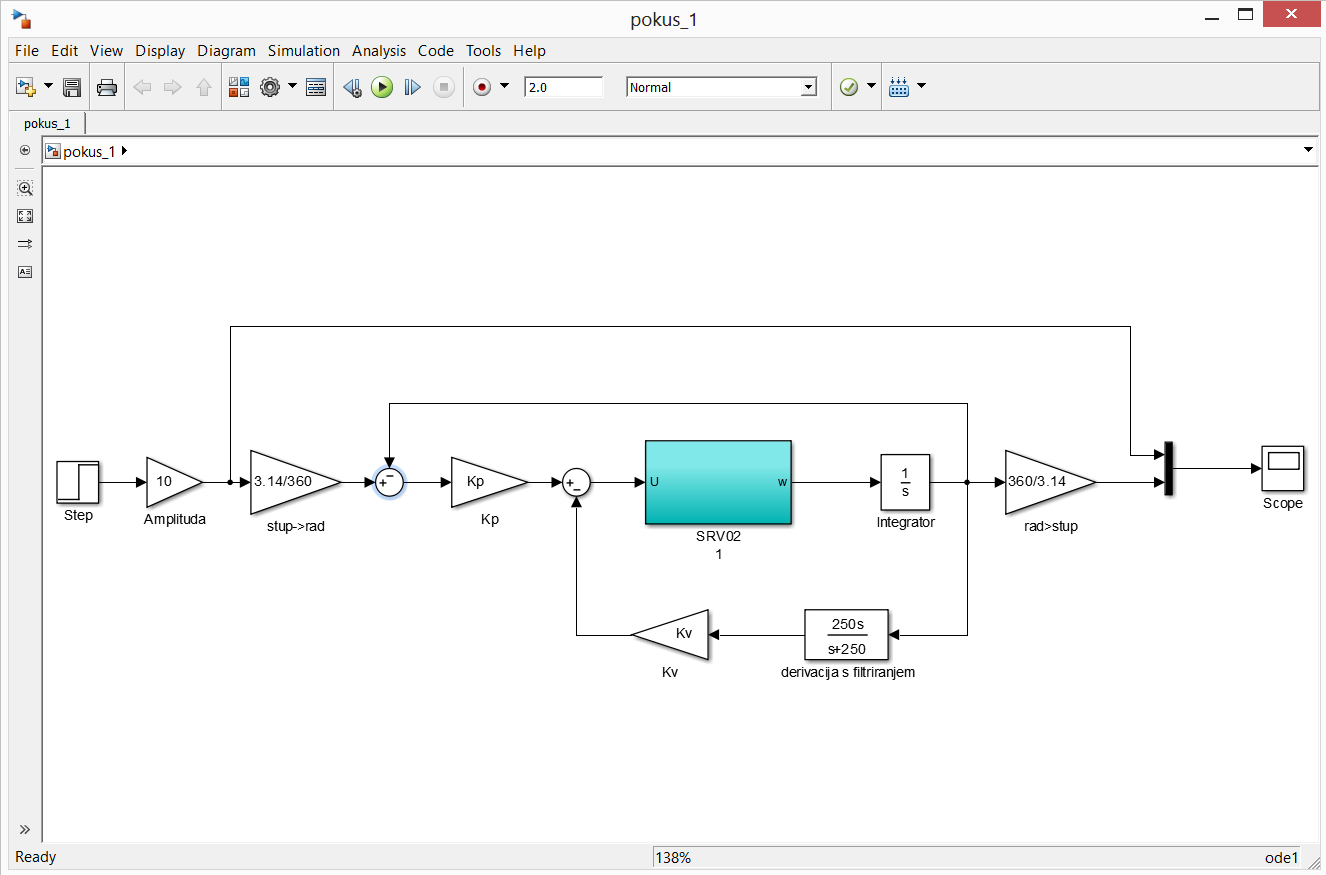
\includegraphics[width=0.8\textwidth] {Simulator.png}
    \caption{Simulacijski model sustava regulacije pozicije rotacijskog elektromehaničkog modula SRV02}
    \end{center}
\end{figure}

Snimamo karakteristične odzive na skokovitu pobudnu funkciju uz različite postavke parametara da bi potvrdili valjanost projektiranih parametara regulatora. Na mjestu standardnog derivacijskog člana u povratnoj vezi PV regulatora, nalazi se derivacijski član s filtrom kojem je zadatak eliminiranje visokofrekventnih smetnji koje dolaze sa strane pogona. Takve visokofrekventne smetnje kod dužih djelovanja mogu štetno utjecati na namot motora. 
Derivacijski član korišten u povratnoj vezi PV regulatora ne može biti idealan jer tada ne bi mogli ostvariti simulaciju i rad u realnom vremenu, zbog nekauzalnosti takvog sustava.

\newpage

\subsubsection{Rezultati simulacije}

U simulaciji uspoređujemo signale pozicije, odnosno kuta zakreta, rotacijskog elektromehaničkog modula SRV02, gdje kao ulaznu pobudu imamo step funkciju, a kao izlaznu imamo odziv našeg reguliranog procesa na referentnu step funkciju.

Slijedi više mjerenja i prikaza rezultata odziva sustava za razne varijacije u parametrima sustava.

\begin{figure}[h]
	\begin{center}
	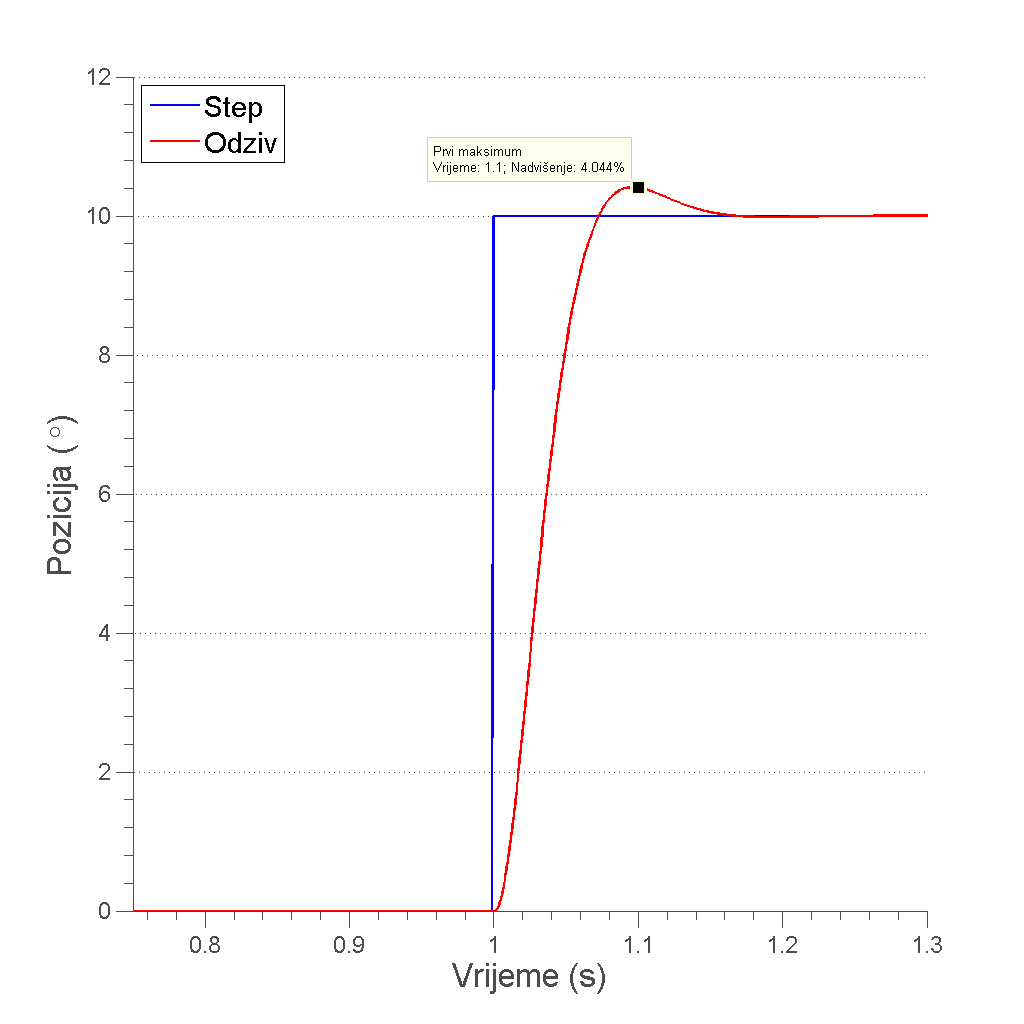
\includegraphics[width=0.8\textwidth] {odziv_1.png}
    \caption{Odziv reguliranog sustava na skokovitu pobudu}
    \end{center}
\end{figure}


Na slici 2.5 možemo vidjeti odziv sustava pri amplitudi ulazne step funkcije iznosa 10 stupnjeva.

Prema očekivanjima, sustav dobro prati zadane zahtjeve, te se prvi maksimum događa nakon približno 100 ms i nadvišenje iznosi otprilike 4\%. Vrijednosti nisu savršeno precizne iz razloga što se u povratnoj petlji regulatora koristi derivator s filtriranjem umjesto pretpostavljenog idealnog derivatora pri proračunu parametara.

\newpage


\begin{figure}[h]
	\begin{center}
	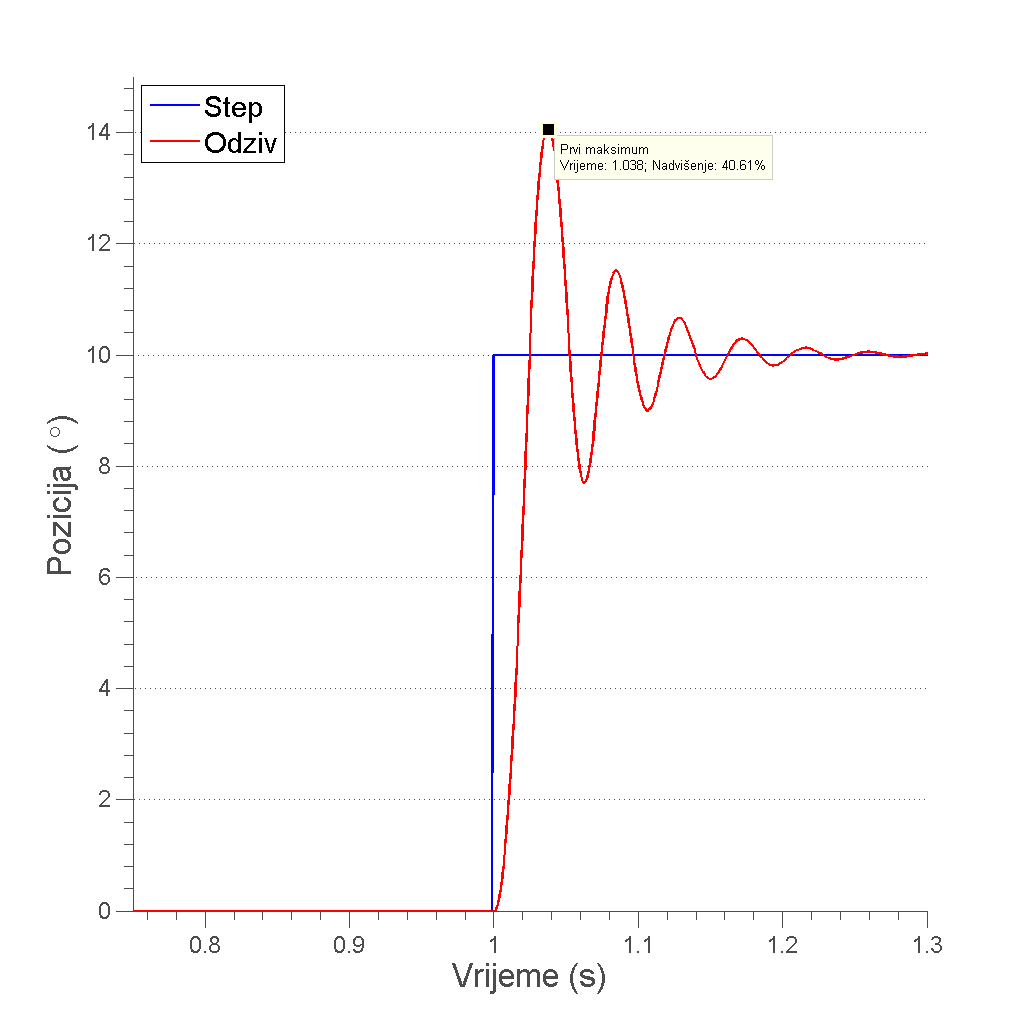
\includegraphics[width=0.8\textwidth] {odziv_2.png}
    \caption{Odziv reguliranog sustava na skokovitu pobudu pri pojačanju $K_p$ 10 puta većeg iznosa }
    \end{center}
\end{figure}

Odziv sustava u situaciji kada je pojačanje $K_p$ deset puta većeg iznosa no proračunatog, odnosno $K_p = 293.399$ dobivamo prema slici 2.6.

Kako promjena iznosa pojačanja $K_p$ nužno za posljedicu povlači narušavanje kvalitete regulatora sustava, dobivamo novo vrijeme prvog maksimuma koje se sada skratilo i iznosi približno 40 ms, te se nadvišenje sustava povećalo na približno 40\%. 

Naravno, takve promjene su u skladu s očekivanjima s obzirom da se pojačanje $K_p$ odnosi proporcionalno prirodnoj frekvenciji $\omega_n$ i obrnuto proporcionalno prigušenju $\zeta$. Prigušenje $\zeta$ direktno utječe na iznos nadvišenja $\varsigma_m$, te s manjim utjecajem prigušenja $\zeta$ u jednadžbi (2-12) nadvišenje biva proporcionalno većeg iznosa. Vrijeme prvog maksimuma $t_p$ ovisi i o prigušenju $\zeta$ i o prirodnoj frekvenciji $\omega_n$, no povećanje prirodne frekvencije $\omega_n$ i smanjenje prigušenja $\zeta$ oboje uvjetuju smanjenje vremena prvog maksimuma, te se takav efekt i vidi u odzivu sustava.



\newpage

Ukoliko sustavu postavimo iznos pojačanja $K_v$ koje je deset puta veće no ono koje smo proračunali, odvija se obrnuti proces negoli onaj koji smo mogli promatrati na slici 2.7.

Sustav postaje tromiji i sličniji sustavu prvoga reda. Postizanje vremena prvog maksimuma se postiže zamjetno sporije, te se očekivano nadvišenje smanjuje do te mjere da praktički ne postoji.

Odziv sustava u takvim uvjetima možemo vidjeti na slici 2.8, te se isti dobiva za  pojačanja iznosa $K_v = 3.643$.

\begin{figure}[h]
	\begin{center}
	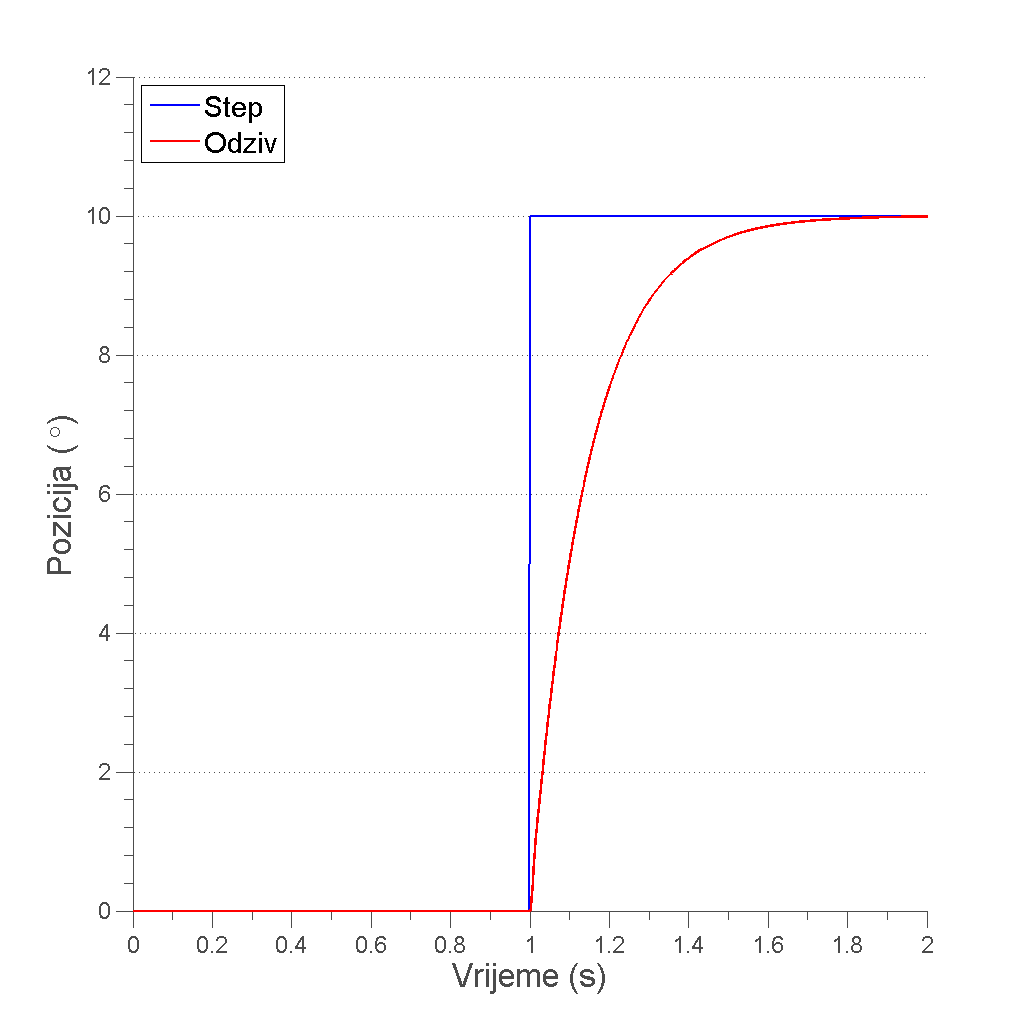
\includegraphics[width=0.8\textwidth] {odziv_3.png}
    \caption{Odziv reguliranog sustava na skokovitu pobudu pri pojačanju $K_v$ 10 puta većeg iznosa }
    \end{center}
\end{figure}


U nastavku slijede odzivi sustava kada imamo pozitivnu povratnu vezu, odnosno kada imamo sustav bez povratne veze

\newpage

\begin{figure}[h!]
	\begin{center}
	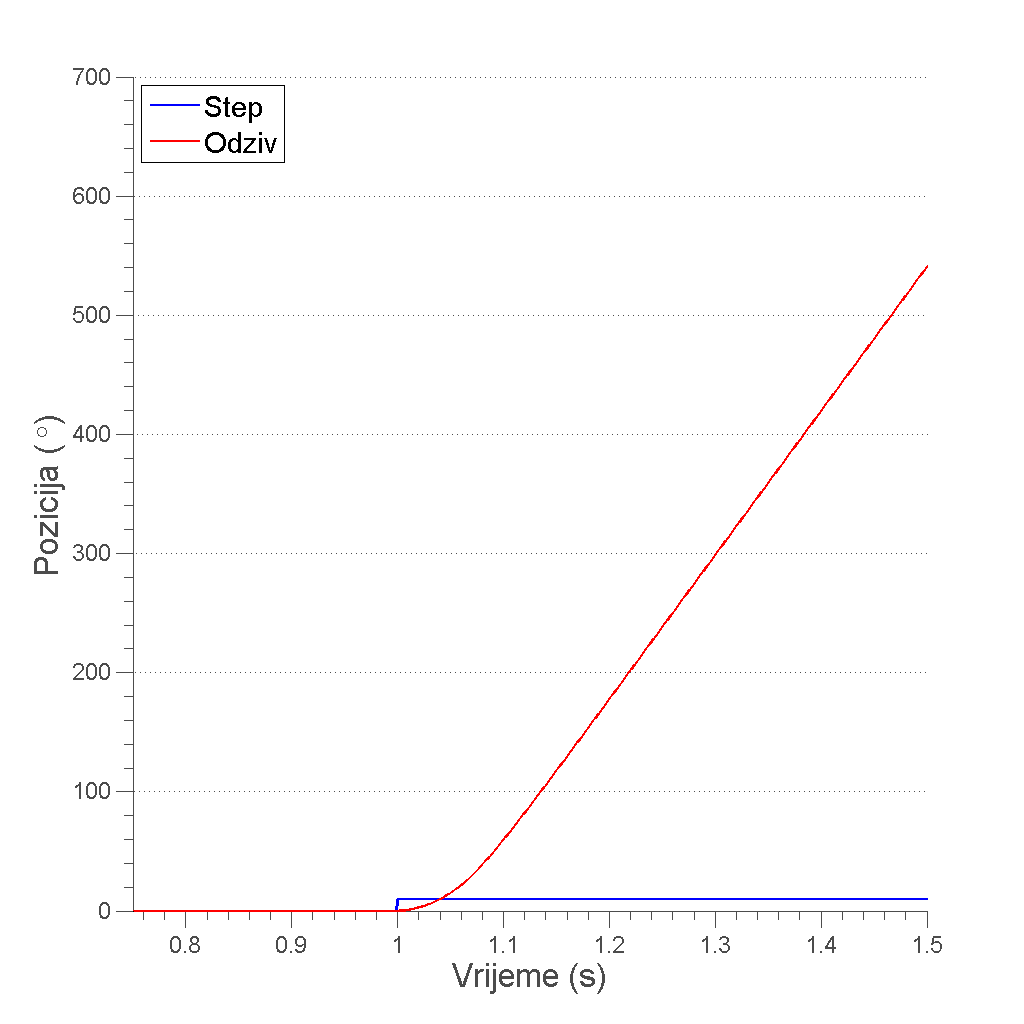
\includegraphics[width=0.8\textwidth, height = 4in] {odziv_pozitivna_povratna.png}
    \caption{Odziv reguliranog sustava na skokovitu pobudu s pozitivnom povratnom vezom }
    \end{center}
\end{figure}



\begin{figure}[h!]
	\begin{center}
	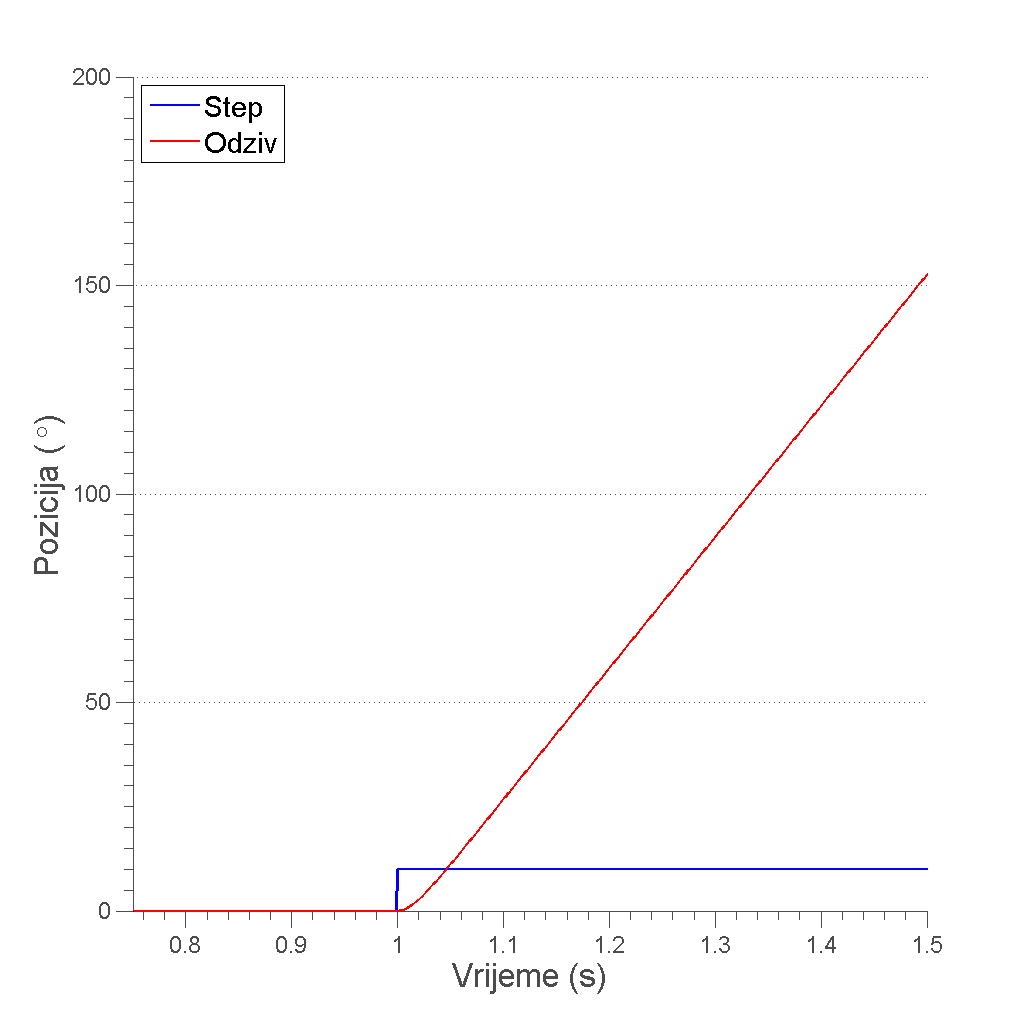
\includegraphics[width=0.8\textwidth, height = 4in] {odziv_bez_povratne.png}
    \caption{Odziv reguliranog sustava na skokovitu pobudu bez povratne veze }
    \end{center}
\end{figure}

\newpage

Kao što možemo primjetiti prema odzivima na slikama 2.8 i 2.9, sustavi s pozitivnom povratnom vezom ili sustavi bez povratne veze za ovakav tip regulatora su inherentno nestabilni, stoga su neupotrebljivi za potrebe naših zahtjeva regulacije.
\newline


Ukoliko mijenjamo amplitudu regulacijske veličine, primjerice na polovinu nominalne amplitude, dobivamo odaziv kao što je prikazan na slici 2.10.

\begin{figure}[h]
	\begin{center}
	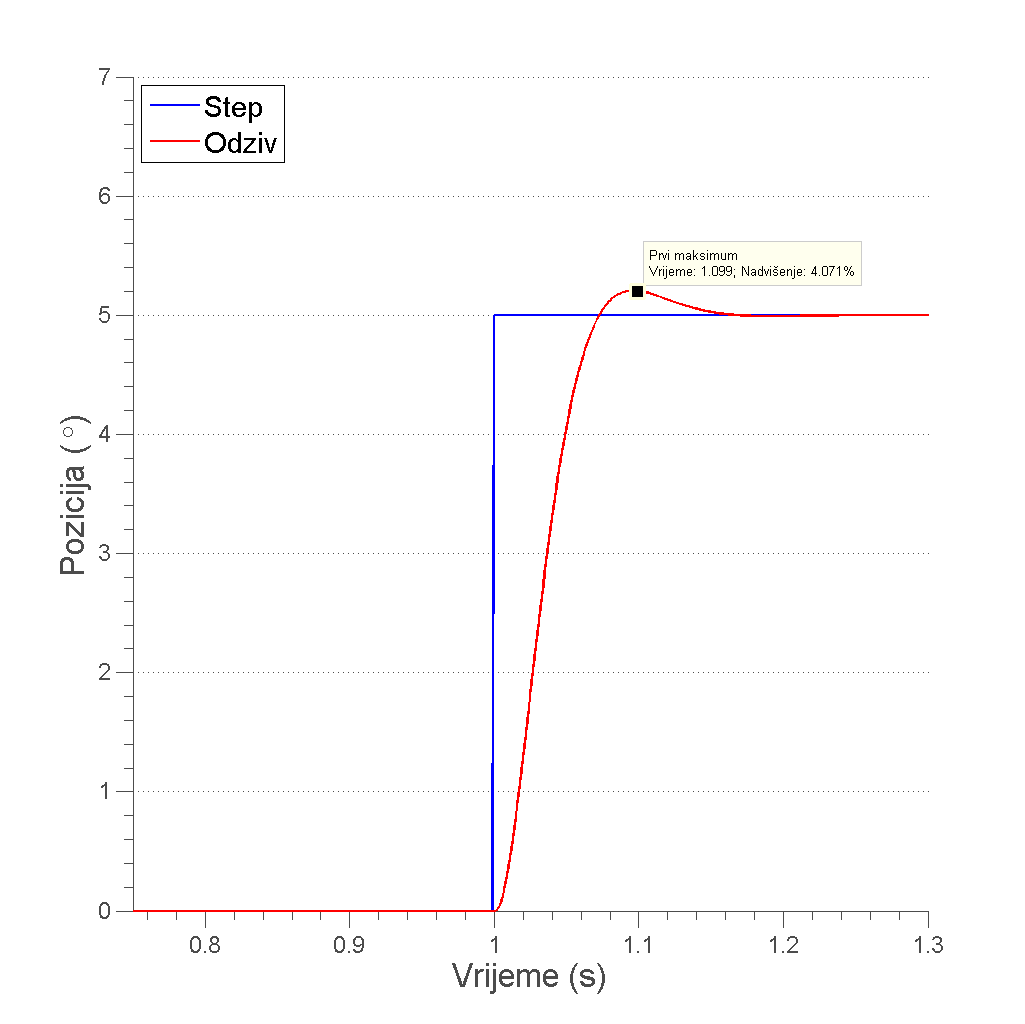
\includegraphics[width=0.8\textwidth] {odziv_pola_nominalne.png}
    \caption{Odziv reguliranog sustava na skokovitu pobudu pri amplitudi iznosa 5 stupnjeva }
    \end{center}
\end{figure}

Ukoliko usporedimo odziv sustava na ovakvu pobudu i odziv sustava prikazan na slici 2.5, primjećujemo da promjena amplitude nije bitno utjecala na regulacijske parametre. Vrijeme prvog maksimuma i iznos prigušenja su ostali isti kao i u primjeru s amplitudom iznosa 10 stupnjeva. Time zaključujemo da kvaliteta našeg regulatora ne ovisi o amplitudi ulaznog pobudnog signala.

\newpage

\subsection{Opažanja i zaključci}

U sklopu ove vježbe obavili smo sintezu PV regulatora pozicije rotacijskog elektomehaničkog sustava SVR02 te smo isti testirali i simulirali u sklopu provjere ispravnosti našega regulatora.

Koristeći matematički model modula SVR02 kojeg smo modelirali u drugoj lab. vježbi, regulacijske zahtjeve zadane u poglavlju ~\ref{sec:zahtjevi} te jednadžbe regulacijskog algoritma uspješno smo modelirali PV regulator koji dovoljno dobro prati naše regulacijske zahtjeve.

Usporedbom jednadžbi parametara regulacije i parametara samog regulatora možemo uvidjeti sljedeće odnose među njima:


\begin{itemize}
\item Pojačanje $K_p$ je proporcionalno prirodnoj frekvenciji $\omega_n$, povećanje $K_p$ povlači povećanje $\omega_n$ i obrnuto, prema jednadžbi (2-21a)
\item Pojačanje $K_p$ je obrnuto proporcionalno prigušenju $\zeta$, povećanje $K_p$ povlači smanjenje $\zeta$ i obrnuto, prema jednadžbi (2-21a)
\item Pojačanje $K_v$ je proporcionalno prigušenju $\zeta$, povećanje $K_p$ povlači povećanje $\zeta$ i obrnuto, prema jednadžbi (2-21b)
\end{itemize}

Naravno, takve promjene su u skladu s rezultatima i odzivima koje smo dobili tokom simulacije.

Primjećujemo da se naš regulirani sustav, s parametrima regulatora $K_p$ i $K_v$ koje smo dobili sintezom, dobro vlada i pri nominalnim iznosima amplitude koje smo zadali na početku simulacije, te pri drugim iznosima, što nas dovodi do zaključka da je kvaliteta naše regulacije neovisna o iznosu amplitude pobudnog signala.

Pri modeliranju matematičkog modela našeg procesa, odnosno rotacijskog elektromehaničkog sustava SRV02, morali smo uzeti par faktora u obzir.

Nelinearni element je dodan u matematički model radi približavanja matematičkog modela stvarnom rotacijskom modulu SRV02, kojemu je rad ograničen na ulazne naponske veličine iznosa od -6 V do 6 V.

Iako je naš matematički modela adekvatan za potrebe naše simulacije, on je u mogućnosti pratiti stvarni rotacijski sustav samo do rezolucije točnosti kojom smo ga mi modelirali. Inherentna ograničenja sustava su promjenjivost parametara modela pri različitim brzinama vrtnje, odnosno različitim iznosima pobudnog signala, zanemarivanje nelinearnosti realnog sustava pri malim iznosima ulaznog signala i slično.

Pri sintezi regulatora pretpostavljeno je da se koristi idealni derivator, dok to nije slučaj u našoj simulaciji gdje koristimo derivator s filtriranjem. Time smo napravili određena zanemarenja koja utječu na naš odziv i vremenske pokazatelje, ali u tolikoj mjeri da ih možemo zanemariti. To smo učinili da bi si olakšali izračun parametara regulatora.


Ukoliko imamo na pameti ograničenja našeg sustava procesa i regulatora, te obratimo pozornost da ispravno tumačimo rezultate. Naš modelirani sustav će adekvatno dobro pratiti zahtjeve regulacije te ujedno i dobro simulirati odaziv kakvog bi očekivali od realnog rotacijskog modula do određene preciznosti.

\end{document}




%Na vlastitu odgovornost...